\section{Costos del Proyecto}
\paragraph{Resumen de costos}

\begin{figure}[htbp]
    \centering
    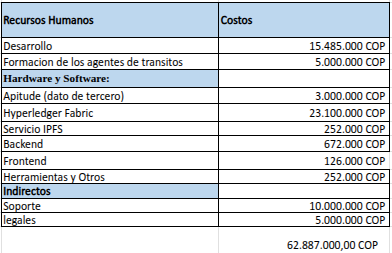
\includegraphics[width=\textwidth]{Images/costos1.png}
    \caption{Resumen de costos del proyecto.}
    \label{fig:costos1}
\end{figure}

Este proyecto involucra el desarrollo e implementación de un sistema de software complejo que utiliza tecnologías modernas como blockchain (Hyperledger Fabric) e IPFS, junto con componentes web tradicionales (React, Express.js). Los costos se han estimado cuidadosamente considerando el esfuerzo de desarrollo, la infraestructura necesaria, la capacitación y otros gastos indirectos. 

En la Figura~\ref{fig:costos1} se presenta un resumen de los costos del proyecto. El costo total estimado asciende a 62.887.000,00 COP. Este monto se desglosa en varias categorías principales que detallaremos a continuación, basándonos en una estimación ascendente del esfuerzo y una proyección de los costos de infraestructura y servicios. 

\paragraph{Costos de Software y Hardware}

\begin{figure}[htbp]
    \centering
    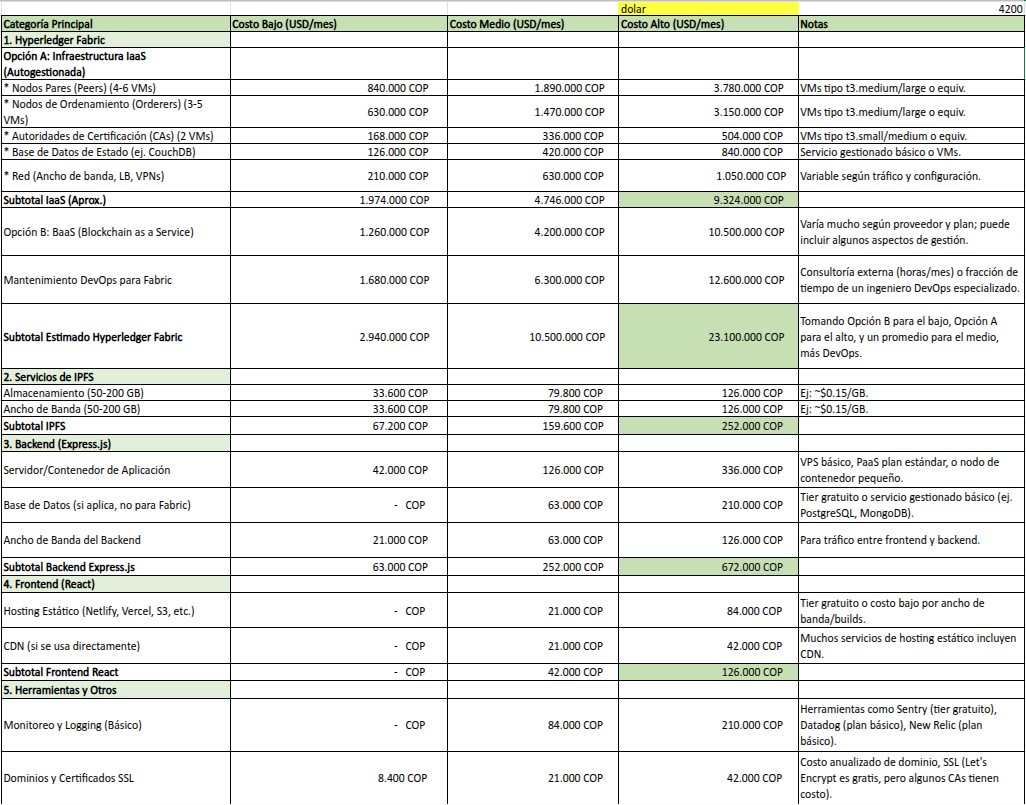
\includegraphics[width=\textwidth]{Images/costos2.png}
    \caption{Estimación de costos mensuales de infraestructura.}
    \label{fig:costos2}
\end{figure}

La Figura~\ref{fig:costos2} proyecta los costos mensuales recurrentes asociados con la infraestructura necesaria para desplegar y operar la aplicación. Ofrece tres escenarios (Bajo, Medio, Alto) para cada componente, reflejando diferentes niveles de capacidad, rendimiento o robustez. Los valores en esta tabla están originalmente en dólares (USD) y se han convertido a pesos colombianos (COP) utilizando una tasa de cambio de 4.200 COP/USD (según la celda indicada). Se ha seleccionado el escenario "Costo Alto (USD/mes)" para alimentar la tabla de "Resumen de Costos". 

\paragraph{Categorías Principales y Subcomponentes (basado en el escenario "Alto" seleccionado): }

\begin{enumerate}
\item \textbf{Hyperledger Fabric:} Es el costo más significativo, reflejando la complejidad de desplegar y mantener una red blockchain permisionada. 

\begin{itemize}
\item \textbf{Infraestructura IaaS (Autogestionada) o BaaS:} Incluye servidores para nodos pares, nodos de ordenamiento, autoridades de certificación, bases de datos de estado y costos de red. El escenario alto seleccionado suma 9.324.000 COP. 

\item \textbf{Mantenimiento DevOps para Fabric:} Un costo crucial para la operación, monitoreo y actualización de la red Fabric, estimado en 12.600.000 COP. 

\item\textbf{Subtotal Estimado Hyperledger Fabric:} 23.100.000 COP (Nota: parece haber una pequeña diferencia entre la suma de los componentes IaaS y DevOps, y el subtotal. El subtotal de 23.100.000 COP es el que se traslada al resumen). 
\end{itemize}
\item \textbf{Servicios de IPFS:} Costos asociados al almacenamiento y ancho de banda para el 		sistema de archivos descentralizado, estimados en 252.000 COP. 

\item \textbf{Backend (Express.js):} Costos del servidor de aplicación, base de datos (si aplica fuera de Fabric) y ancho de banda para la API, sumando 672.000 COP. 

\item \textbf{Frontend (React):} Costos de hosting estático y CDN para la interfaz de usuario, estimados en 126.000 COP. 

\item \textbf{Herramientas y Otros:} Incluye monitoreo, logging, dominios y certificados SSL, con un costo de 252.000 COP. 
\end{enumerate}
 

\textbf{GRAN TOTAL ESTIMADO MENSUAL (Escenario Alto):} El costo mensual recurrente total para la infraestructura y servicios, en el escenario alto, es de 24.402.000 COP. Nota: Este es el costo mensual. En la tabla de resumen de costos, algunos de estos se presentan como si fueran un costo único o para un periodo específico, lo cual habría que aclarar (ej. si el costo de Hyperledger Fabric de 23.100.000 COP es para el primer mes, o para un periodo de setup y algunos meses de operación). Si es mensual, el total del proyecto se dispararía si es para muchos meses. 

\medskip
\textit{Nota del equipo de proyecto:} Este capítulo permanecerá provisionalmente para fines de trazabilidad. Se contempla su eliminación o reemplazo por un anexo financiero detallado en versiones futuras, una vez se definan los modelos de despliegue y financiación definitivos.

\paragraph{Costo de Desarrollo }
\begin{figure}[htbp]
    \centering
    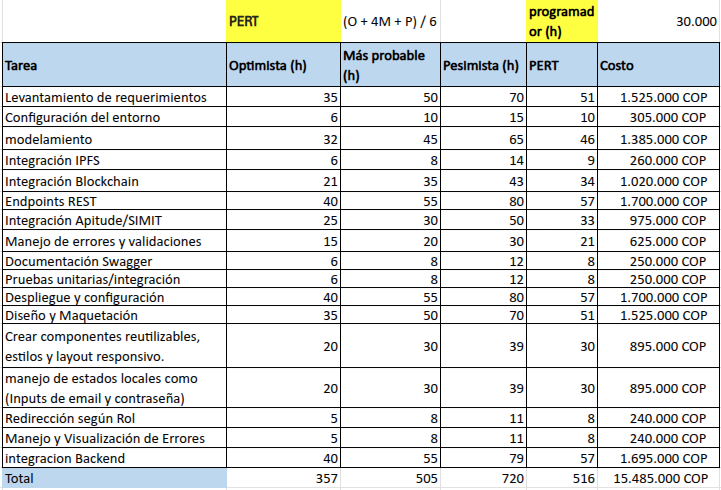
\includegraphics[width=\textwidth]{Images/costos3.png}
    \caption{Estimación de costos de desarrollo del proyecto.}
    \label{fig:costos3}
\end{figure}

La Figura~\ref{fig:costos3} detalla el esfuerzo estimado para cada tarea específica del desarrollo del software. Utiliza la técnica PERT (Program Evaluation and Review Technique) para calcular un tiempo ponderado (columna "PERT (h)") basándose en estimaciones optimistas, más probables y pesimistas. Este esfuerzo en horas se traduce luego en un costo, asumiendo una tarifa por hora de programador de 30.000 COP (según la celda "programador (h)"). 
\paragraph{Columnas Clave: }
\begin{itemize}
\item \textbf{Tarea:} Describe las actividades individuales de desarrollo, desde el levantamiento de requerimientos hasta el despliegue y diseño. 

\item \textbf{Optimista (h), Más probable (h), Pesimista (h):} Son las tres estimaciones de tiempo para cada tarea, fundamentales para la técnica PERT. 

\item \textbf{PERT (h): }Es el tiempo estimado ponderado calculado con la fórmula (Optimista + 4 * Más probable + Pesimista) / 6. Este valor representa una estimación más realista del tiempo que tomará cada tarea, considerando la incertidumbre. 

\item \textbf{Costo}: Es el resultado de multiplicar las horas PERT por la tarifa horaria del programador (30.000 COP). 
\end{itemize}
 

\paragraph{Total de Desarrollo:} El costo total de desarrollo de software asciende a 15.485.000 COP, correspondiente a un esfuerzo total estimado de 516 horas PERT. Esto cubre todas las fases del ciclo de vida del desarrollo, incluyendo la integración con IPFS, Blockchain, el desarrollo de Endpoints REST, pruebas, y la creación de la interfaz de usuario. 